% !TEX TS-program = XeLaTeX
% use the following command: 
% all document files must be coded in UTF-8
\documentclass{textolivre}
% for anonymous submission
%\documentclass[anonymous]{textolivre}
% to create HTML use 
%\documentclass{textolivre-html}
% See more information on the repository: https://github.com/leolca/textolivre

% Metadata
\begin{filecontents*}[overwrite]{article.xmpdata}
    \Title{Impact of ICT on writing and reading skills: a systematic review (2010-2020)}
    \Author{José María Fernández Batanero \sep Marta Montenegro Rueda \sep José Fernández Cerero \sep }
    \Language{en}
    \Keywords{ICT \sep Writing \sep Reading \sep Review}
    \Journaltitle{Texto Livre}
    \Journalnumber{1983-3652}
    \Volume{14}
    \Issue{2}
    \Firstpage{1}
    \Lastpage{12}
    \Doi{10.35699/1983-3652.2021.34055}

    \setRGBcolorprofile{sRGB_IEC61966-2-1_black_scaled.icc}
            {sRGB_IEC61966-2-1_black_scaled}
            {sRGB IEC61966 v2.1 with black scaling}
            {http://www.color.org}
\end{filecontents*}

% used to create dummy text for the template file
\definecolor{dark-gray}{gray}{0.35} % color used to display dummy texts
\usepackage{lipsum}
\SetLipsumParListSurrounders{\colorlet{oldcolor}{.}\color{dark-gray}}{\color{oldcolor}}

% used here only to provide the XeLaTeX and BibTeX logos
\usepackage{hologo}

% used in this example to provide source code environment
%\crefname{lstlisting}{lista}{listas}
%\Crefname{lstlisting}{Lista}{Listas}
%\usepackage{listings}
%\renewcommand\lstlistingname{Lista}
%\lstset{language=bash,
        breaklines=true,
        basicstyle=\linespread{1}\small\ttfamily,
        numbers=none,xleftmargin=0.5cm,
        frame=none,
        framexleftmargin=0.5em,
        framexrightmargin=0.5em,
        showstringspaces=false,
        upquote=true,
        commentstyle=\color{gray},
        literate=%
           {á}{{\'a}}1 {é}{{\'e}}1 {í}{{\'i}}1 {ó}{{\'o}}1 {ú}{{\'u}}1 
           {à}{{\`a}}1 {è}{{\`e}}1 {ì}{{\`i}}1 {ò}{{\`o}}1 {ù}{{\`u}}1
           {ã}{{\~a}}1 {ẽ}{{\~e}}1 {ĩ}{{\~i}}1 {õ}{{\~o}}1 {ũ}{{\~u}}1
           {â}{{\^a}}1 {ê}{{\^e}}1 {î}{{\^i}}1 {ô}{{\^o}}1 {û}{{\^u}}1
           {ä}{{\"a}}1 {ë}{{\"e}}1 {ï}{{\"i}}1 {ö}{{\"o}}1 {ü}{{\"u}}1
           {Á}{{\'A}}1 {É}{{\'E}}1 {Í}{{\'I}}1 {Ó}{{\'O}}1 {Ú}{{\'U}}1
           {À}{{\`A}}1 {È}{{\`E}}1 {Ì}{{\`I}}1 {Ò}{{\`O}}1 {Ù}{{\`U}}1
           {Ã}{{\~A}}1 {Ẽ}{{\~E}}1 {Ũ}{{\~u}}1 {Õ}{{\~O}}1 {Ũ}{{\~U}}1
           {Â}{{\^A}}1 {Ê}{{\^E}}1 {Î}{{\^I}}1 {Ô}{{\^O}}1 {Û}{{\^U}}1
           {Ä}{{\"A}}1 {Ë}{{\"E}}1 {Ï}{{\"I}}1 {Ö}{{\"O}}1 {Ü}{{\"U}}1
           {ç}{{\c{c}}}1 {Ç}{{\c{C}}}1
}


\journalname{Texto Livre}
\thevolume{14}
\thenumber{2}
\theyear{2021}
\receiveddate{\DTMdisplaydate{2020}{12}{11}{-1}} % YYYY MM DD
\accepteddate{\DTMdisplaydate{2021}{02}{28}{-1}}
\publisheddate{\DTMdisplaydate{2021}{7}{8}{-1}}
% Corresponding author
\corrauthor{José María Fernández Batanero}
% DOI
\articledoi{10.35699/1983-3652.2021.34055}
%\articleid{NNNN} % if the article ID is not the last 5 numbers of its DOI, provide it using \articleid{} commmand
% list of available sesscions in the journal: articles, dossier, reports, essays, reviews, interviews, editorial
\articlesessionname{dossier}
% Abbreviated author list for the running footer
\runningauthor{Fernández Batanero et al.}
\editorname{Anna Izabella M. Pereira}

\title{Impact of ICT on writing and reading skills: a systematic review (2010-2020)}
\othertitle{Impacto das TIC nas habilidades de escrita e leitura: uma revisão sistemática (2010-2020)}
% if there is a third language title, add here:
%\othertitle{Artikelvorlage zur Einreichung beim Texto Livre Journal}

\author[1]{José María Fernández Batanero~\orcid{0000-0003-4097-5382}~\thanks{Email: \url{batanero@us.es}}}
\author[1]{Marta Montenegro Rueda~\orcid{0000-0003-4733-289X}~\thanks{Email: \url{mmontenegro1@us.es}}}
\author[1]{José Fernández Cerero~\orcid{0000-0002-2745-6986}~\thanks{Email: \url{jfcerero@us.es}}}
\author[1]{Pedro Román Gravan~\orcid{0000-0002-1646-9247}~\thanks{Email: \url{proman@us.es}}}

\affil[1]{Universidad de Sevilla, Facultad de Ciencias de la Educación, Departamento de Didáctica y Organización Educativa, Sevilla, España.}

\addbibresource{article.bib}
% use biber instead of bibtex
% $ biber tl-article-template

% set language of the article
\setdefaultlanguage{english}
\setotherlanguage{portuguese}

% for spanish, use:
%\setdefaultlanguage{spanish}
%\gappto\captionsspanish{\renewcommand{\tablename}{Tabla}} % use 'Tabla' instead of 'Cuadro'
%\AfterEndPreamble{\crefname{table}{tabla}{tablas}\Crefname{table}{Tabla}{Tablas}}

% for languages that use special fonts, you must provide the typeface that will be used
%\setotherlanguage{russian}
%\newfontfamily\russianfont{Literaturnaya}
% \newfontfamily\arabicfontsf[Script=Arabic]{Amiri}
% \newfontfamily\arabicfonttt[Script=Arabic]{Amiri}
%
% in the article, to add arabic text use: \textlang{arabic}{ ... }

% for russian text we also need to define fonts with support for Cyrillic script
% in the text use \begin{russian} ... \end{russian}
\usepackage{fontspec}
\setotherlanguage{russian}
\newfontfamily\cyrillicfont{Times New Roman}
\newfontfamily\cyrillicfontsf{Times New Roman}[Script=Cyrillic]
\newfontfamily\cyrillicfonttt{Times New Roman}[Script=Cyrillic]

% to use emoticons in your manuscript
% https://stackoverflow.com/questions/190145/how-to-insert-emoticons-in-latex/57076064
% using font Symbola, which has full support
% the font may be downloaded at:
% https://dn-works.com/ufas/
% add to preamble:
% \newfontfamily\Symbola{Symbola}
% in the text use:
% {\Symbola }

% reference itens in a descriptive list using their labels instead of numbers
% insert the code below in the preambule:
\makeatletter
\let\orgdescriptionlabel\descriptionlabel
\renewcommand*{\descriptionlabel}[1]{%
  \let\orglabel\label
  \let\label\@gobble
  \phantomsection
  \edef\@currentlabel{#1\unskip}%
  \let\label\orglabel
  \orgdescriptionlabel{#1}%
}
\makeatother
%
% in your document, use as illustraded here:
%\begin{description}
%  \item[first\label{itm1}] this is only an example;
%  % ...  add more items
%\end{description}
 

% custom epigraph - BEGIN 
%%% https://tex.stackexchange.com/questions/193178/specific-epigraph-style
\usepackage{epigraph}
\renewcommand\textflush{flushright}
\makeatletter
\newlength\epitextskip
\pretocmd{\@epitext}{\em}{}{}
\apptocmd{\@epitext}{\em}{}{}
\patchcmd{\epigraph}{\@epitext{#1}\\}{\@epitext{#1}\\[\epitextskip]}{}{}
\makeatother
\setlength\epigraphrule{0pt}
\setlength\epitextskip{0.5ex}
\setlength\epigraphwidth{.7\textwidth}
% custom epigraph - END


% if you use multirows in a table, include the multirow package
\usepackage{multirow}

% add line numbers for submission
%\usepackage{lineno}
%\linenumbers

\begin{document}
\maketitle

\begin{polyabstract}
\begin{abstract}
Due to the potential of ICT to enhance the development of reading and writing skills, it has become an emerging field of scientific research. This paper aims examine scientific literature that investigates the use of ICT in the development of writing and reading skills for the years 2010 and 2020 in five databases. A descriptive and quantitative methodology has been followed to present the most important characteristics and results of the 16 selected scientific articles. In analysis of the research findings we explored the most significant bibliometric data and the effectiveness of ICTs in enhancing the writing and reading skill of students. The results confirmed that, despite the fact that scientific production in this field is still underdeveloped, digital technologies can help in the development of reading and writing skills. There is a need to improve teacher training for the effective integration of technologies in both teaching and learning of reading and writing.

\keywords{ICT \sep Writing \sep Reading \sep Systematic review}
\end{abstract}

\begin{portuguese}
\begin{abstract}
Devido ao potencial das TIC para melhorar o desenvolvimento das capacidades de leitura e escrita, tornou-se um campo emergente da investigação científica. O objectivo deste trabalho tem sido examinar a literatura científica que investiga o uso das TIC no desenvolvimento de competências de escrita e leitura para os anos 2010 e 2020 em cinco bases de dados. Foi seguida uma metodologia descritiva e quantitativa para apresentar as características e resultados mais importantes dos 16 artigos científicos seleccionados. Na análise dos resultados da investigação explorámos os dados bibliométricos mais significativos e a eficácia das TIC na melhoria da capacidade de escrita e de leitura dos estudantes. Os resultados confirmaram que, apesar de a produção científica neste campo estar ainda subdesenvolvida, as tecnologias digitais podem ajudar no desenvolvimento das capacidades de leitura e de escrita. Há necessidade de melhorar a formação de professores para a integração eficaz das tecnologias tanto no ensino como na aprendizagem da leitura e da escrita.

\keywords{TIC \sep Escrita \sep Leitura \sep Revisão sistemática}
\end{abstract}
\end{portuguese}

% if there is another abstract, insert it here using the same scheme
\end{polyabstract}


\section{Introduction}\label{sec-intro}
The modern era is characterized by the use of technological tools in an extensive diversity of their daily activities, especially those of telecommunications and information technology: e-mail, chat, blogs, social networks, video games, among others. This social model implies transformations in social, cultural and economic relations, as well as changes in the communication ways enabled by the development of technology and the media or instruments used. Screens are replacing paper while keyboards are replacing pencils, which has modified the usual structure of text and its reading compared to the printed version \cite{cordongarcia2015}. These changes are reflected in the field of education, as somewhat, they have to report on how they influence students' lifestyles. More than a decade ago, authors such as \textcite{kress2005} explained the need to think about education based on changes such as the shift from writing to screen and the preeminence of images. Similarly, many authors \cite{godoy2017, sandberg2015} point out that new reading and writing practices have emerged with the transformations in digital communication. Thus, \textcite{cassany2011} and \textcite{magadan2014} pointed out as advantageous not only the potential of ICTs and the Internet in the field of literacy, but also in terms of text distribution, which multiplies the number of potential readers and providing spaces for the dissemination of their own materials.

Reading comprehension is a purposeful process, in which the reader has an active role and employs cognitive skills that must be developed through strategies that are teachable and can be enhanced through practice over time \cite{vandijk1983}. This suggests that developing reading, comprehension and discursive production skills in people is necessary both for creating meaning and communicative purposes. In this regard, current literature has raised the need to change the way we think about reading comprehension and the production of discourse influenced by Technology.
 
The ICTs provide essential support in the teaching-learning processes of reading and writing skills, which has resulted in a field of scientific research. At present, thanks to technological resources, it has become an emerging field of study. Thus, using Google Trends a tool that enables the analysis of search trends in a browser, to assess the frequency of the terms "ICT", "reading" and "writing" in the world over the last decade, and it is possible to observe a constant percentage of searches. In the academic field, the growth is greater, with a quick search on Google Scholar using the terms "Literacy and ICT" revealing more than 10,000 results for the period 1990 to 2020. However, while it is likely that not all of these articles are related to ICT use and literacy, the high number of results identified suggests that there is a growing interest in this field of research.

\textcite{navarrete2015} presented a review of research conducted in Latin America, focusing on technologies such as the strengthening reading comprehension and the production of written discourse in middle school students, during the period 2002-2014. The information obtained made it possible to review the studies and organize them into two categories; one related to the use and appropriation of ICT in the development of reading skills, and the other is related to proposals aimed at strengthening discursive production based on the incorporation of ICTs in the classroom. Regarding the methodology, most of the studies are framed in the qualitative approach, only three of these papers correspond to studies of experimental approach with pretest, intervention and postest.

Concerning ICTs in teaching-learning processes of reading comprehension, the results from the study by \textcite{coiro2007}, which suggest that prior knowledge and skills are necessary to be successful in reading experiences on the Internet. The English-speaking context also highlights the positive effects on the development of reading-skills supported by ICTs \cite{schneider2016}. However, other authors such as \textcite{andrews2003} or \textcite{voogt2007}, found that the use of ICT to develop literacy shows positive effects.

Recently, a study on literacy development through ICT \cite{suarezcardenas2015} has shown that ICTs develop literacy skills and promote students` learning because these skills are covered in the learning across different knowledge areas. Teachers also play a key role in the development of literacy through ICT support \cite{avidov-ungar2018}. 

\section{Theorical Background}
Language is directly linked to educational success, as all educational activities are communicative and therefore comprehension isclosely linked to communicative competence. Reading/writing is not exclusive to the language area, because it becomes a support for learning, because reading and writing allow for dialogue, sharing and verification of knowledge; access and production of written information \cite{bautistavillalobos2015}. Reading and writing have always had a special significance and importance at school. Authors such as \textcite{lerner2001} argue that these two terms represent the most essential school function, a reason that drives its analysis in order to redefine its meaning within the school context and foster a literacy culture among students. Reading and writing are processes that involve a set of operations at the thinking level. For \textcite{alvarez_rol_1987}, reading and writing is placed in the comprehension and production texts processes, where a set of non-serial mental operations appear in dynamics. In other words, these operations are simultaneous or parallel so that students may understand the information they are exposed to.

Moreover, \textcite{castillo2010} define bibliometrics as "a part of scientometrics that applies mathematical and statistical methods to all scientific literature and the authors who produce it, with the aim of studying and analysing scientific activity" (p.3). According to \textcite{licea2002}, scientific bibliometrics is a research field that nowadays holds a very relevant influence for journals and researchers. It was used for decades to measure scientific activity and impact. Nowadays there are many studies focused on measuring scientific production in different areas and this interest has generated this type of studies.

Taking into account the progress made in ICT, and educational experiences to improve students' reading and writing skills, we consider it is necessary to analyse the scientific literature in this field in the last decade (2010-2020). The purpose of this paper is to examine the impact of technology on the development of students' reading and writing skills. We assessed the results of these resources in the latest research to reveal to the scientifict commnunity the progress and upcoming trends in the literature about reading and writing through the use of ICTs.

In this regard, the following research questions are proposed:

\begin{itemize}
\item What is the general state of the scientific literature in the field of ICT for the development of students' reading and writing skills?
\item If technology is used to teach reading and writing, what are the learning outcomes for students?
\item What are the main lines of research in the field of ICT and reading and writing development?
\end{itemize}

\section{Material and Method}
\subsection{Procedure}
The purpose of this paper is to carry out a systematic review of the scientific literature published between: 2010-2020. In this study, we have reviewed the papers that analyse the impact of ICT to promote the development of reading and writing processes, following the guidelines established in education for bibliometric studies \cite{fernandezcano1998}. For this purpose, descriptive and quantitative methods were applied, as well as the technique of network maps for the analysis of keywords \cite{knoke2007}, which have been visually represented through the VOSviewer tool. In addition, this research was based on the criteria for systematic reviews established in PRISMA statement \cite{moher2009}.

For data analysis, bibliometric analysis of keywords in the field were used \cite{bhattacharya2003, ding2001, chiu2005, lopez2015} through co-occurrence analysis within the research field \cite{cahlik2000, viedmadeljesus2011}.

\subsection{Search Strategy}
For the systematic literature search, we selected five databases [N=259]: WoS, Scopus, ERIC, SciELO and Google Scholar, through the use of the keyword search strategy. This review was conducted in February 2021. Searches were limited to articles published between 2010 and 2020, containing the combination of the descriptors (ICT, reading and writing) in the title, abstract and/or keywords.

In order to determine which studies would be collected, a set of criteria were established. These criteria were established by the authors. Among the inclusion criteria, the following were specified: a) Published between 2010 and 2020; b) Combination of descriptors in the title, abstract or keywords; c) Published in peer-reviewed journals; d) Related to the education sciences. The exclusion criteria include: a) type of document (scientific articles only); b) studies published in non-periodical publications; c) documents that are not addressing the use of ICTs as a way of learning from reading and writing, and d) duplicate entries. Following a review, the number of articles was reduced to [N=109].

The 109 articles were full-text reviewed for eligibility, thus 93 articles were excluded for the following reasons: a) they were not related to the field of education and b) the type of document. As a result, 14 articles met the eligibility criteria (N=16). The results are summarised in a flow chart following the PRISMA guidelines \cite{moher2009} (\Cref{fig1}).

\begin{figure}[htbp]
 \centering
 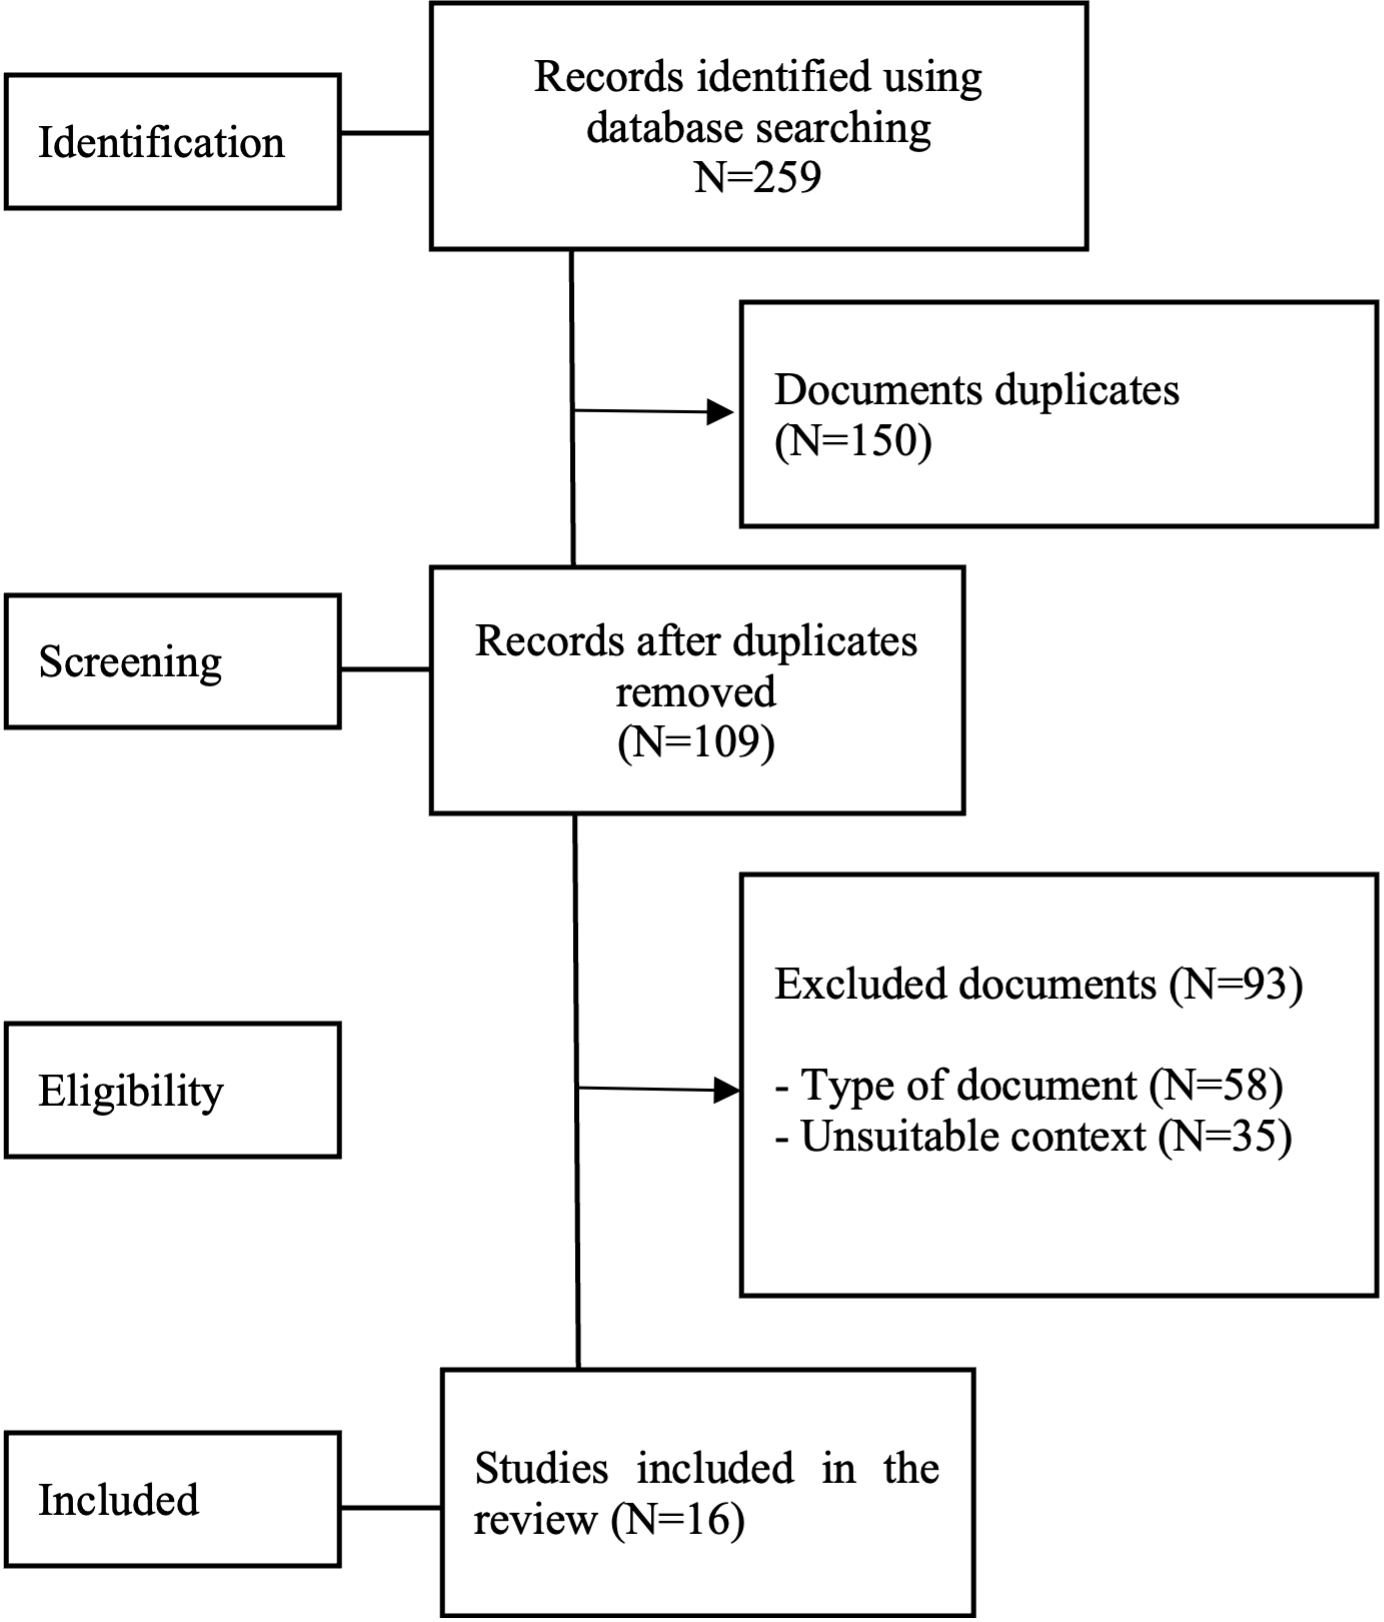
\includegraphics[width=0.65\textwidth]{fig-001.png}
 \caption{Flowchart according to the PRISMA declaration.}
 \label{fig1}
 \source{own elaboration.}
\end{figure}

\subsection{Data extraction}
The purpose of this paper was to select studies that present an overview of the research, extracting (a) research objectives, (b) student data, (c) methodology, (d) use of technology, and (e) learning outcomes, among other aspects \cite{wu2012}.  Thus, the authors have conducted a manual task after analysing and reviewing the selected studies.

\section{Results}
Below, the results are presented in two phases. On the one hand, quantitative data are presented to answer the first objective of the research. On the other hand, the keyword graphs and their analysis are presented in order to identify the main lines of research in this field.

\subsection{Phase 1. Main characteristics and findings of selected studies}
In this systematic review of the literature, 16 articles have been extracted from the different databases analysed. The selected articles, produced between 2010-2020, aimed to assess the impact of ICT use on the development of reading and writing skills. \Cref{fig2} shows the distribution of the studies published in this period. The highest number of selected articles is found in 2019 and 2020, which reveals that the production on ICT and literacy is increasing in the last years.

\begin{figure}[htbp]
 \centering
 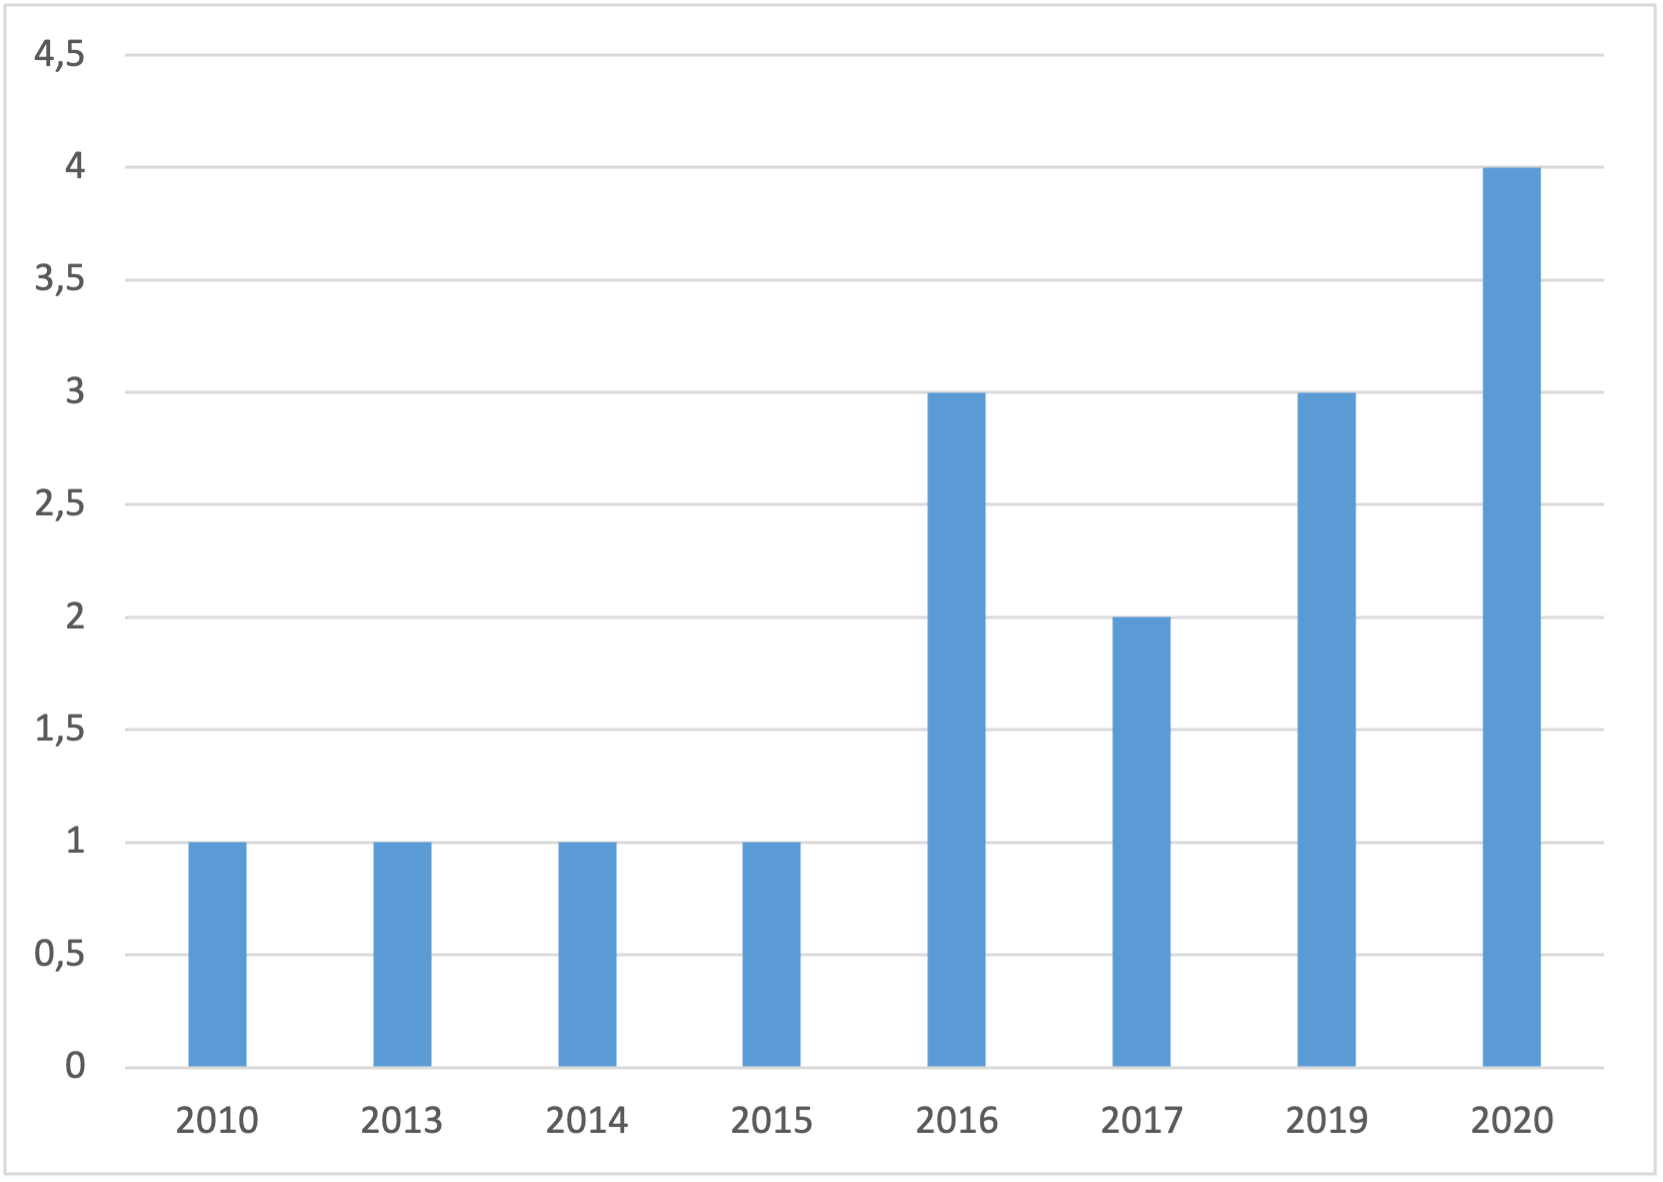
\includegraphics[width=0.65\textwidth]{fig-002.png}
 \caption{Study distribution between years 2010-2020.}
 \label{fig2}
 \source{own elaboration.}
\end{figure}

All studies are summarized in \Cref{tab1}. Four of the 16 studies analyzed recommended the use of ICT for students with autism and other intellectual disabilities \cite{bailey2016, felix2017, weiser2019, badillo-jimenez2020}. All the studies have been developed within the educational field and in any educational stage. We find that most of them focus on primary education (81.25\%). Studies aimed at secondary education (12.5\%) and university education (6.25\%) are minor.

\begin{longtable}{p{0.17\textwidth}p{0.13\textwidth}p{0.12\textwidth}p{0.1\textwidth}p{0.09\textwidth}p{0.22\textwidth}}
\caption{Analysis of the selected studies.}
\label{tab1}
\\
\toprule
Study & Methodology & Resource used & Student & Country & Results
\\
\midrule
\textcite{montelongo2010} & Theory & ICT & Higher Education & United States & Technology encourages improved comprehension of reading and writing
\\
\textcite{genlott2013} & Quantitative & iWTR method (ICT) & Primary Education & Sweden & ICT improved reading and writing skills
\\
\textcite{zhong2014} & Quantitative & ICT & University Education & United States & ICT improves your skills, knowledge and motivation
\\
\textcite{neirapineiro2015} & Qualitative & Blogs (Internet) & Higher Education & Spain & A literature blog enhances
\\
\textcite{bailey2016} & Quantitative & Computer-assisted program & Primary Education & Australia & Improved reading comprehension of students with autism
\\
\textcite{keane2016} & Theory & ICT & All students & Australia & ICT can improve reading and writing skills but must be used appropriately
\\
\textcite{costa2016} & Quantitative & E-Book & Primary Education & Brazil & E-book contributed significantly of learning reading, writing and the development of various skills
\\
\textcite{andrade2017} & Theory & ICT & Primary Education & Venezuela & ICT is creating new enjoyable activities
for reading and
writing
\\
\textcite{felix2017} & Quantitative & Computer-assisted program & Primary Education & Mexico & This tool is effective
in supporting
learning for children
with intellectual
disabilities
\\
\textcite{liu2019} & Quantitative & ICT & Primary Education
& 
Taiwan & It is recommended to
use ICT to promote
reading from 12
years
\\
\textcite{polihronov2019} & Quantitative & Pedagogical technology
&
Primary
Education
& 
Bulgaria & Fosters skills like
listening, reading,
speaking, and writing
\\
\textcite{weiser2019} & Quantitative & Coaching through
&
Primary
Education
&
United
States
&
Promotes the
development of technology reading, writing and
spelling skills of
people with learning
difficulties

\\
\textcite{badillo-jimenez2020} & Theory & Interactive story (ICT)
&
Primary
Education
&
Colombia & Interactive story
(TIC) enhance
reading
comprehension in
autistic stude
\\
\textcite{gozukucuk2020} & Quantitative & Computer-assisted program & Primary Education
&
Turkey & These activities
improved reading
comprehension
\\
\textcite{hautala2020} & Quantitative & Computer-assisted program (Digital Games)
&
Primary
Education
&
Finland & Educational games
with technology help
improve the
development of
reading skills
\\
\textcite{luna2020} & Qualitatitve & iPad & Primary Education & United States & iPads encourage motivation and learning
\\
\bottomrule
\source{own elaboration.}
\end{longtable}

In the analysis of the content areas of the publications, we can divide them into reading and writing processes. Thus, 6 papers focused on reading skills (37.5\%), one of them focused on writing skills (6.25\%), and nine studies included both reading and writing skills development (56.25\%).

The results obtained, from the analysis of the methodologies used, reveal that the main part of the research is those studies that have focused on a quantitative methodology (62.5\%), followed by those that have an imminently theoretical approach (25\%). To a lesser extent there are those that have a higher qualitative focus (12.5\%). The methodological approach of the articles is a valuable tool that provides an overview of how ICT research and reading and writing are being addressed in the scientific literature.

In the analysis of the countries that have shown the greatest activity posting on the selected topic, during the last decade, United States (25\%) and Australia (12.5\%) stand out. In \Cref{fig3}, it can be seen that research in the field of ICT to support literacy in reading and writing is a global issue.


\begin{figure}[htbp]
 \centering
 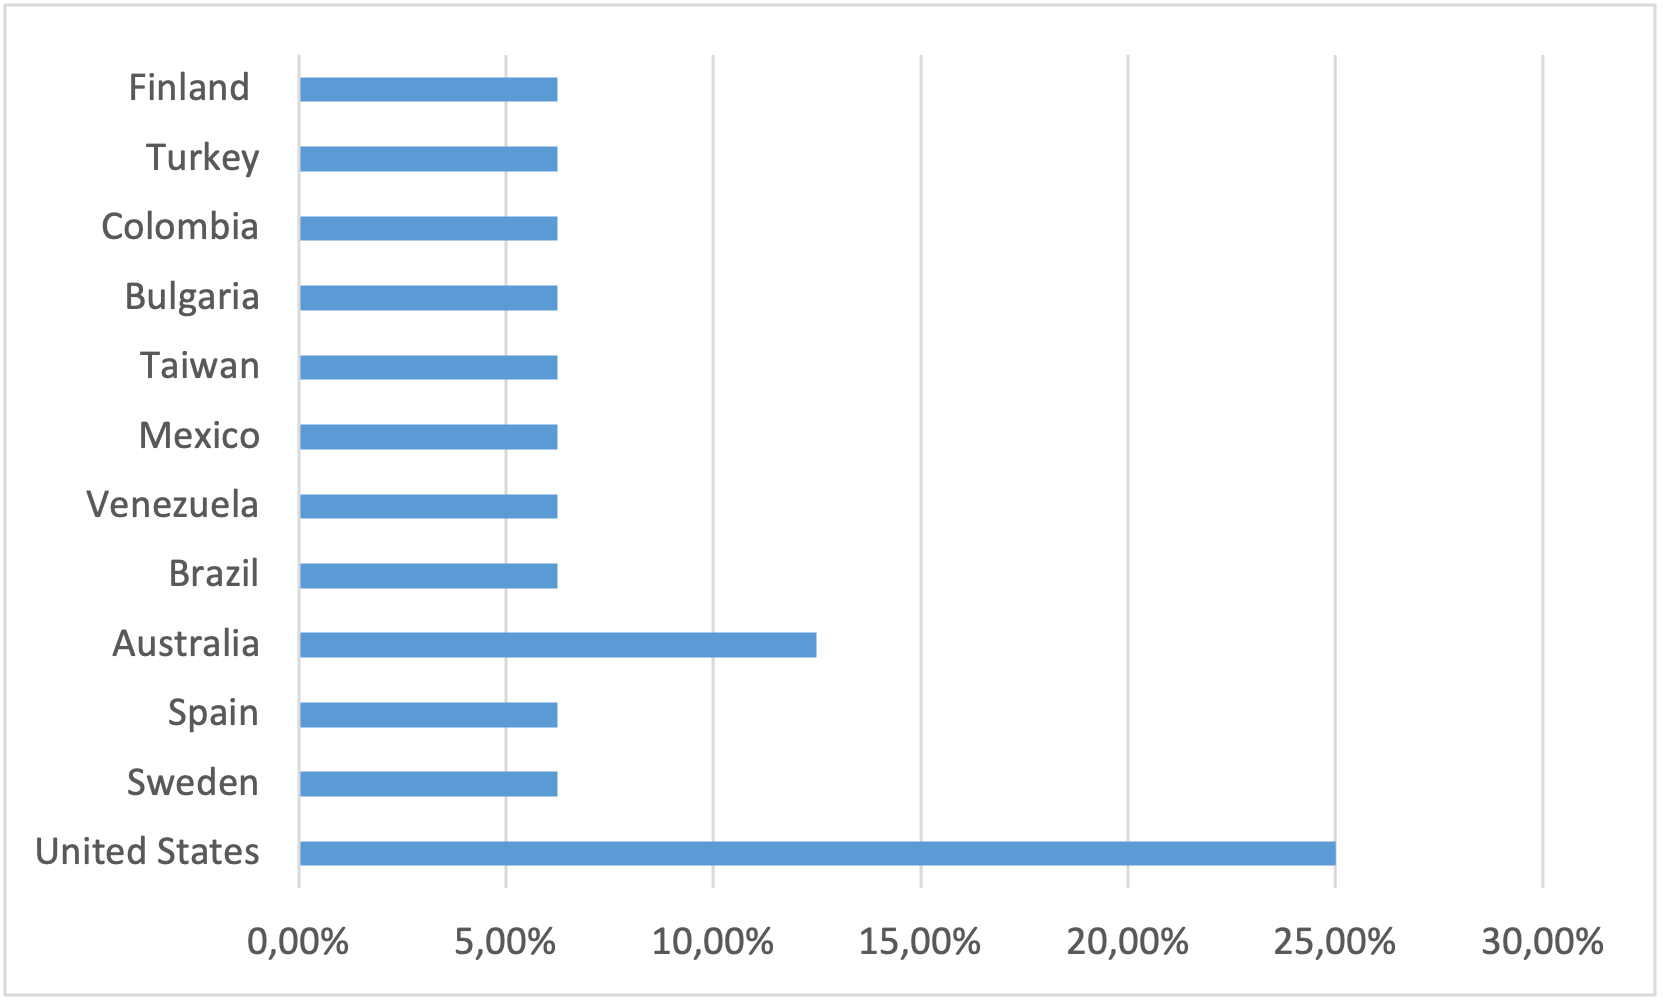
\includegraphics[width=0.7\textwidth]{fig-003.png}
 \caption{Percentage of articles by country.}
 \label{fig3}
 \source{own elaboration.}
\end{figure}

Concerning the type of ICT tools most used, various categories are established. Firstly, computers (50\%), mainly for the use of educational programmes, the use of Blogs or the use of the Internet. Secondly, there are tablets or iPads (25\%), which are mainly used for the use of playful applications and educational software based on playing as a learning method. Finally, there are digital games (12.5\%) and electronic books (12.5\%), through which interactive reading is encouraged. These are innovative tools for promoting reading skills. 

\subsection{Phase 2. Analysis of Keyword Relationships}
Next, in order to identify possible trends and research directions, an analysis of the relationships of the keywords used in the documents has been carried out.

For this purpose, the VosViewer software was used, which is a tool for the construction of bibliometric networks that allows to know the relation of the key words "Key-Words Plus (KW+)" that have been identified in the area of study. In order to understand the labelled bibliometric map (\Cref{fig4}), it is important to know in advance whether the map extracts the keywords most frequently from the selected documents and it establishes the relationship between them. The size of the labels (node) is proportional to their weight. In other words, to their appearance frequency. The colour shows the thematic group, or cluster, to which each keyword (KW+) belongs.

In order to obtain the bibliometric map, the 16 studies selected for the review were analysed, from which a total of 235 keywords were extracted. After analysing the homogeneity, 4 groups (clusters) were formed according to the level of similarity (\Cref{fig4}).

\begin{figure}[htbp]
 \centering
 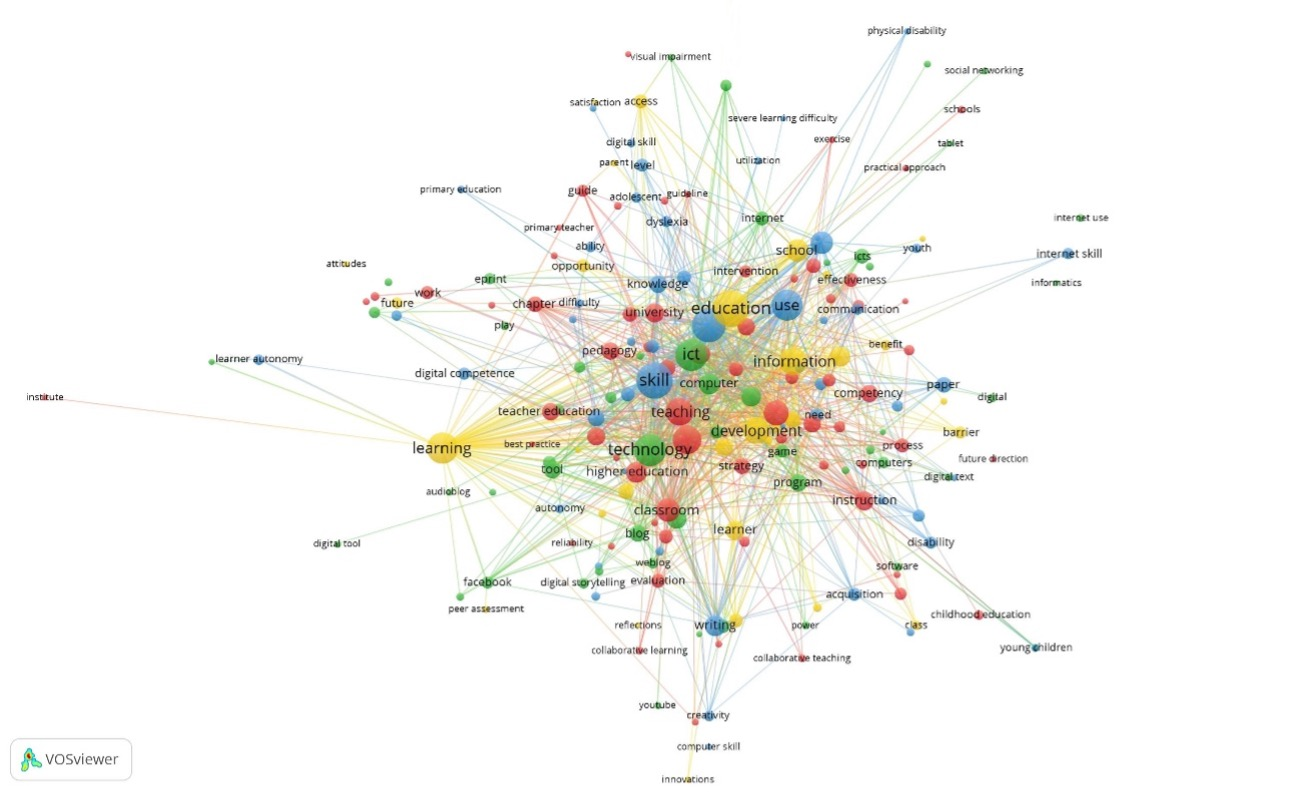
\includegraphics[width=0.85\textwidth]{fig-004.jpg}
 \caption{Bibliometric map Tagged.}
 \label{fig4}
 \source{own elaboration.}
\end{figure}

The four clusters obtained define the main research trends:

Cluster 1 (green): it includes the ICT resources used in the classroom for learning to read and write. This cluster groups 60 items. The most important items are: ICT (193), technology (193), computer (193), web (60). 

Cluster 2 (red): it focuses on the teacher's role in applying ICT in the classroom. This cluster included 57 items such as: teacher (147), practice (108), classroom (83), reading and writing skills (50).

Cluster 3 (blue): it relates to learner characteristics and the importance of integrating ICT in the teaching-learning process. This cluster groups 53 items such as: learner (259), ability (221), use (175), and knowledge (42).

Cluster 4 (yellow): it is related to inclusive educational practice, teacher training and family involvement. Training is essential for the successful implementation of educational practices. This cluster groups 50 items. The most important are: training (270), information (183), experience (135) and learning (58).

\section{Discussion and conclusions}
Responding to the first research question (Q1), related to the general state of research on ICT in support of literacy, the main conclusion is that the production of scientific literature during the last decade is still underdeveloped. This is reflected in the small number of articles published in journals indexed in the selected databases. The scarcity of research poses a problem for the use of ICT for reading and writing processes. In order to easily integrate these tools in the classroom, teachers need to be aware through scientific literature of the multiple benefits they offer, as well as adequate digital competence. Although the countries with the highest scientific output in this field are the United States and Australia, it is a field which, as the results show, is developing all over the world.

In relation to the research designs that prevail in studies on ICT and reading and writing skills, we can highlight that most of the publications developed a quantitative methodology, coinciding with the study carried out by \textcite{periathiruvadi2012}.

In relation to the second question (Q2), we can affirm that the results in students` learning when using ICT for reading and writing are extensive. It has been observed that among the good practices carried out with ICTs to support reading and writing there are no significant differences between countries. Educational innovation through the use of technology has offered good practices in the school environment worldwide. Among the main positive factors that promote the use of these resources are enjoyment, the acquisition of knowledge and motivation \cite{montelongo2010, zhong2014}.  

Technological devices in the classroom, such as the computer, electronic books or iPad, have the potential to influence students` learning in a positive way.  We can highlight the experiences offered in schools in the United States where they have invested in digital tools, such as the iPad, to achieve better learning \cite{luna2020}. The main tool used in the studies analysed is the computer. Therefore, we recommend that teachers use computer-based reading texts with visual support to improve students' reading comprehension \cite{gozukucuk2020}.

E-books, as well as interactive stories or online reading, contribute significantly to the advancement of learning to read, write and develop different skills, as well as to achieve the autonomy of students \cite{costa2016, liu2019, polihronov2019, badillo-jimenez2020}. Furthermore, we can highlight that the use of digital games favours reading development \cite{hautala2020}.

In addition to these ICT tools, the teaching practices that implement their classes with strategies that require the use of Internet are also highlighted. Blogs \cite{neirapineiro2015} stand out, due to these tools enhance communicative skills in a digital environment and it increases the participants’ motivation and encourages independent learning.

We can mention that digital tools offer opportunities in the literacy of students around the world, but the lack of teacher training is one of the reasons that limit these experiences \cite{genlott2013}. The use of information and communication technologies is essential to develop many skills. However, the mere use of technology does not guarantee that learning will take place, but it must be used properly \cite{keane2016}.

Finally, in relation to the main research lines within the ICT field and literacy learning (Q3) through the visualization of bibliometric map, it should be said that, during the period analysed, studies on ICT and reading and writing are being linked thematically to students with learning difficulties, Down Syndrome or autism \cite{bailey2016, felix2017, weiser2019}. Likewise, there is an emerging issue group related to teacher training in ICT as a tool for learning to read and write. In this regard, the teacher must generate a shift in their pedagogical practice, in order to offer society what is expected in times of information and knowledge globalization \cite{andrade2017}. 

Further studies will analyse how ICT can contribute not only to their educational needs, but also to the development of social skills. Thus, we argue for the importance of analysing the potential of ICTs for the teaching-learning processes of reading and writing, because it has not been enough developed.

The limitations found in this study are derived from the small number of published studies and the limited dissemination of empirical studies over the last decade of research in this field.



\printbibliography\label{sec-bib}
% if the text is not in Portuguese, it might be necessary to use the code below instead to print the correct ABNT abbreviations [s.n.], [s.l.] 
%\begin{portuguese}
%\printbibliography[title={Bibliography}]
%\end{portuguese}

\end{document}
